\section{Resultados}
\label{sec:resultados}

En esta sección reportamos los resultados de las 30 ejecuciones por cadena. Primero presentamos la calidad del \textit{gbest} final y su convergencia, después el comportamiento de las tres medidas de diversidad y de los coeficientes, y al final la comparación entre estrategias de coeficientes.

%%%%%%%%%%%%%%%%%%%%%%%%%%%%%%%%%%%%%%%%%%%%%%%%%%%%%
\subsection{Calidad de las soluciones finales}
\label{sec:res_finales}

La Tabla~\ref{tab:gbest_final} resume el \textit{gbest} de la última iteración. Todas las ejecuciones terminaron con una conformación completa, así que el \textit{gbest} es siempre la energía de una conformación válida. El error relativo es $(\bar{E} - E^*)/|E^*|$, donde $\bar{E}$ es la media de las 30 ejecuciones.

\begin{table}[H]
\centering
\caption{\textit{gbest} final en 30 ejecuciones por cadena. ``Éxitos'' cuenta las ejecuciones que alcanzaron la energía mínima conocida, y ``Última mejora'' es la iteración (media $\pm$ desviación estándar) en la que cada ejecución alcanzó su valor final.}
\label{tab:gbest_final}
\small
\setlength{\tabcolsep}{4pt}
\begin{adjustbox}{max width=\textwidth}
\begin{tabular}{lccccccc}
\toprule
Cadena & $E^*$ & Mejor & Peor & Mediana & Media $\pm$ desv. est. & Éxitos & Última mejora \\
\midrule
S1-20 & $-9$  & $-9$  & $-8$  & $-9.0$  & $-8.67 \pm 0.48$  & 20/30 & $59 \pm 49$ \\
S2-24 & $-9$  & $-9$  & $-7$  & $-8.0$  & $-8.17 \pm 0.59$  & 8/30  & $131 \pm 181$ \\
S4-36 & $-14$ & $-14$ & $-11$ & $-12.0$ & $-12.33 \pm 0.96$ & 4/30  & $292 \pm 199$ \\
S5-48 & $-23$ & $-21$ & $-15$ & $-19.0$ & $-18.73 \pm 1.39$ & 0/30  & $558 \pm 192$ \\
S8-64 & $-42$ & $-33$ & $-24$ & $-30.0$ & $-29.73 \pm 2.33$ & 0/30  & $668 \pm 211$ \\
\bottomrule
\end{tabular}
\end{adjustbox}
\end{table}

En las tres cadenas más cortas el algoritmo alcanzó la energía mínima conocida en al menos una ejecución. En S1-20 lo hizo en 20 de las 30, y en las 10 restantes terminó en $-8$, a un solo contacto del óptimo. En S2-24 y S4-36 el óptimo apareció en 8 y 4 ejecuciones, y la mediana quedó uno y dos contactos por arriba. En S5-48 y S8-64 ninguna ejecución llegó al óptimo: la mejor quedó a dos contactos en S5-48 ($-21$ de $-23$) y a nueve en S8-64 ($-33$ de $-42$). El error relativo de la media crece con la longitud: 3.7\,\% en S1-20, 9.3\,\% en S2-24, 11.9\,\% en S4-36, 18.6\,\% en S5-48 y 29.2\,\% en S8-64. La desviación estándar también aumenta, de 0.48 a 2.33, lo que indica que en las cadenas largas el resultado depende más de la ejecución.

La columna de la última mejora muestra una diferencia en el tipo de comportamiento. En S1-20 las ejecuciones alcanzaron su valor final, en promedio, en la iteración 59, y el resto de la ejecución no aportó nada. En S5-48 y S8-64 la última mejora ocurrió en promedio después de la iteración 550, y en varias ejecuciones cerca del final. Esto quiere decir que en las cadenas cortas el algoritmo se detiene porque ya encontró lo que podía encontrar, mientras que en las largas se detiene porque se acabaron las iteraciones.

%%%%%%%%%%%%%%%%%%%%%%%%%%%%%%%%%%%%%%%%%%%%%%%%%%%%%
\subsection{Convergencia del gbest}
\label{sec:convergencia}

La Figura~\ref{fig:convergencia} muestra la media y la desviación estándar del \textit{gbest} en cada iteración. En las cinco cadenas la mayor mejora ocurre en las primeras 50 iteraciones, cuando el enjambre pasa de conformaciones aleatorias a conformaciones con algunos contactos. En S1-20 y S2-24 la curva queda casi plana desde la iteración 200. En S4-36 sigue bajando lentamente hasta la iteración 600. En S5-48 y S8-64 la curva sigue bajando al final de la ejecución, y la pendiente en la segunda mitad es mayor en S8-64, que es la cadena con más margen de mejora.

\begin{figure}[H]
\centering
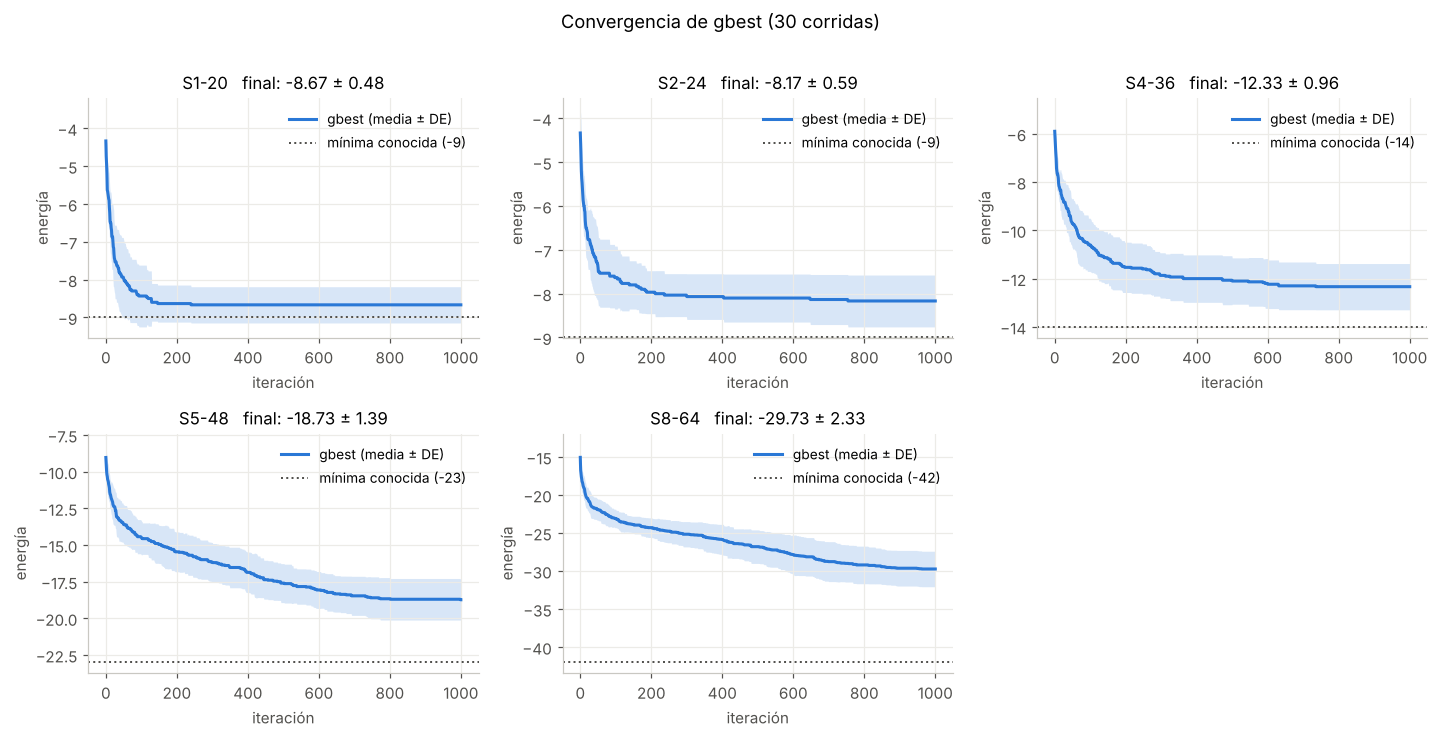
\includegraphics[width=\textwidth]{figuras/hp_convergencia.png}
\caption{Convergencia del \textit{gbest}: media (línea) y $\pm$ una desviación estándar (banda) en 30 ejecuciones. La línea punteada es la energía mínima conocida.}
\label{fig:convergencia}
\end{figure}

La Figura~\ref{fig:plegamientos} muestra la mejor conformación encontrada para cada cadena. En todas se observa lo que predice el modelo: las H forman un núcleo compacto en el centro y las P quedan en la orilla o en lazos hacia afuera. En S8-64 algunos segmentos de H quedan fuera del núcleo, en los extremos de la conformación; cada uno de ellos representa contactos que la conformación no aprovecha, y ayuda a entender la distancia de nueve contactos respecto a la mejor energía conocida.

\begin{figure}[H]
\centering
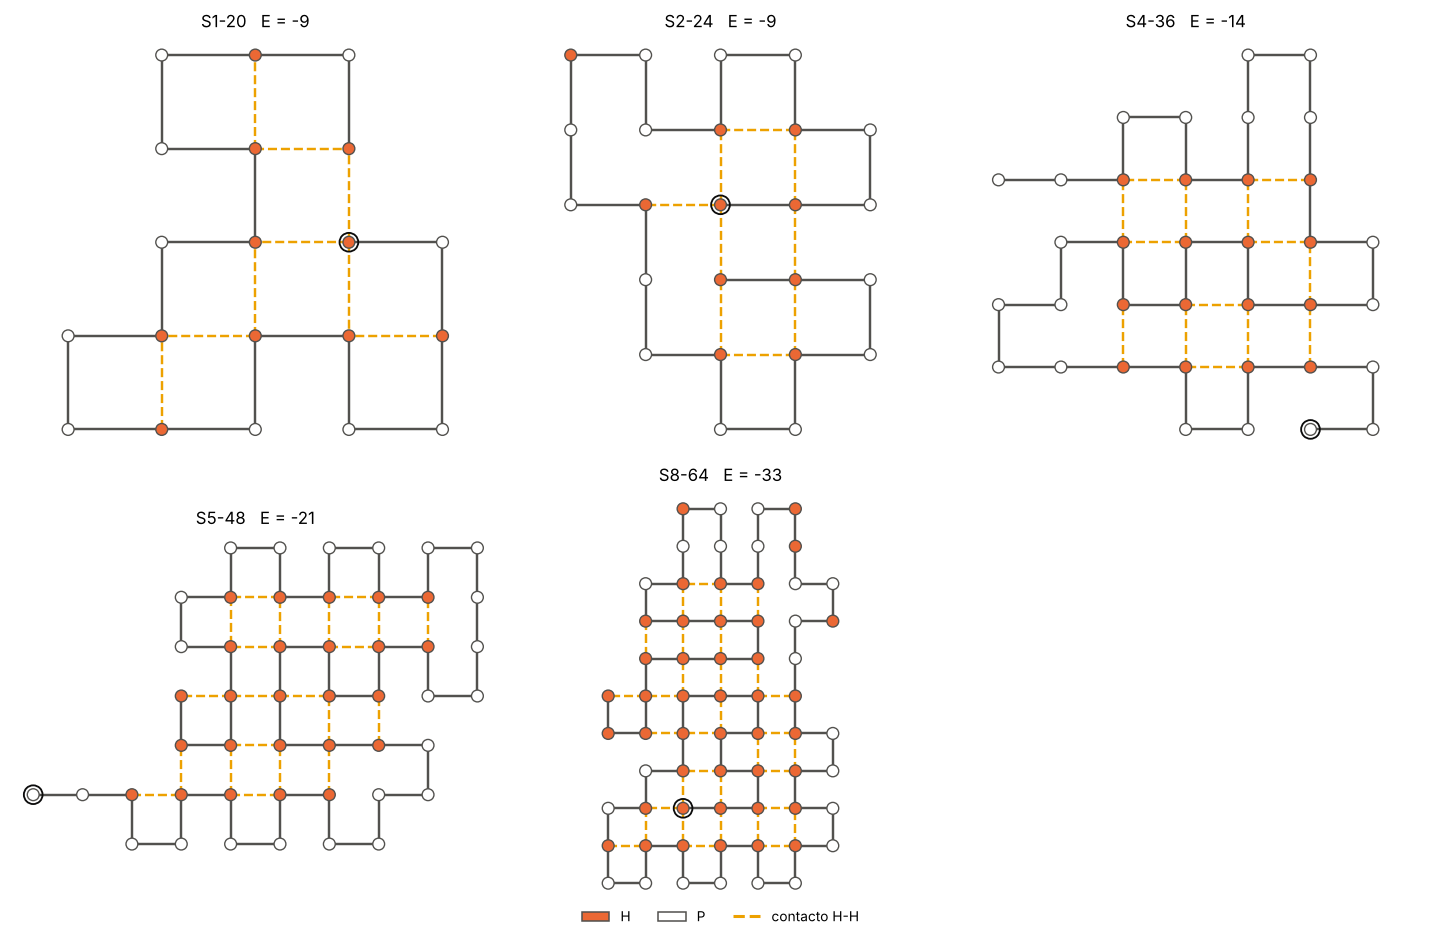
\includegraphics[width=\textwidth]{figuras/hp_mejores_plegamientos.png}
\caption{Mejor conformación encontrada en las 30 ejecuciones de cada cadena. El círculo negro marca el primer aminoácido.}
\label{fig:plegamientos}
\end{figure}

%%%%%%%%%%%%%%%%%%%%%%%%%%%%%%%%%%%%%%%%%%%%%%%%%%%%%
\subsection{Diversidad del enjambre}
\label{sec:res_diversidad}

La Figura~\ref{fig:diversidad} muestra las tres medidas de diversidad para cada cadena, junto con los valores medios de $w$, $c_1$ y $c_2$ que se usaron. La Tabla~\ref{tab:diversidad} da los valores en algunas iteraciones.

\begin{figure}[H]
\centering
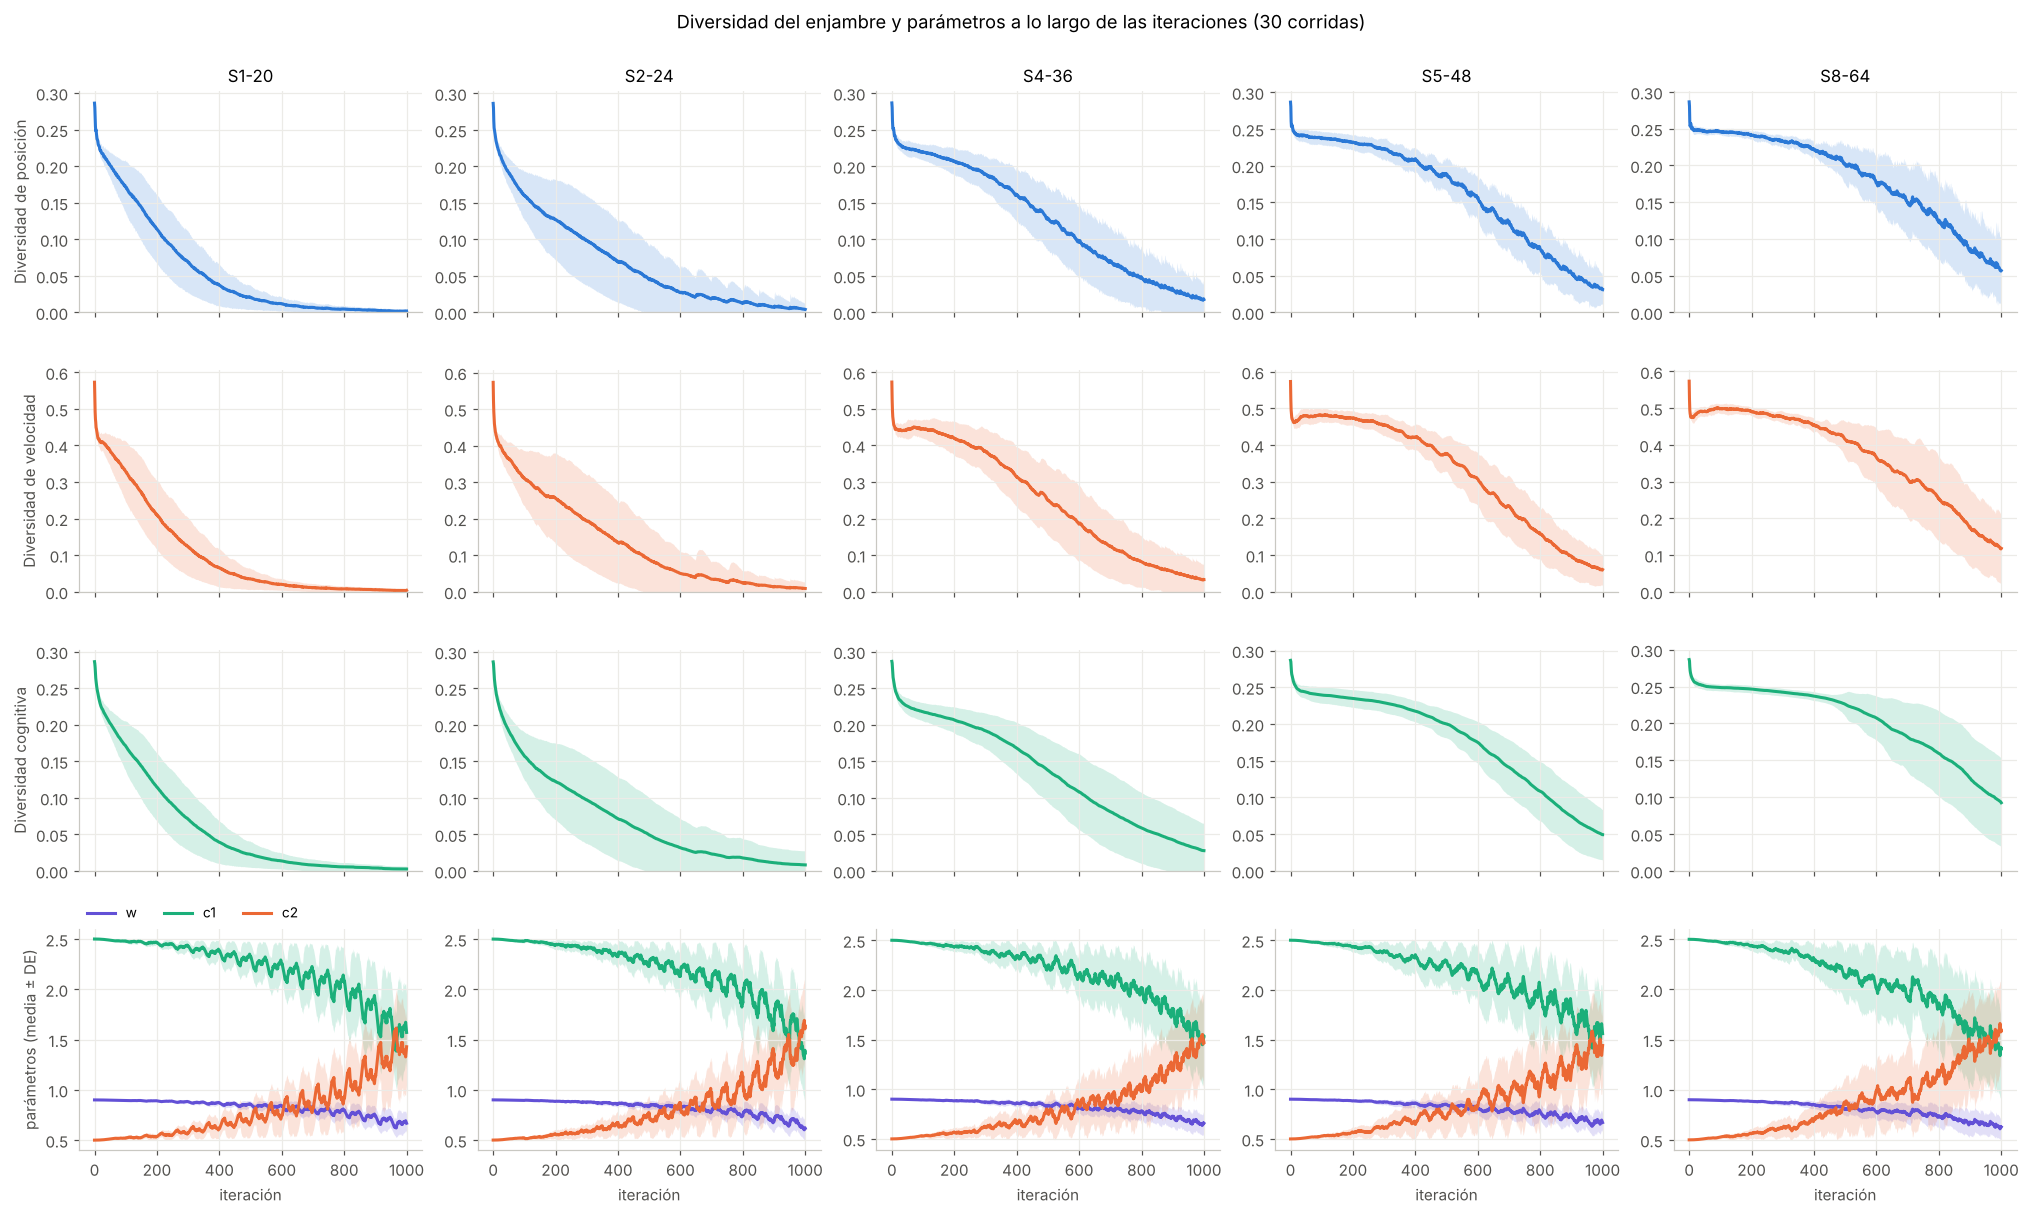
\includegraphics[width=\textwidth]{figuras/hp_diversidad_parametros.png}
\caption{Diversidad de posición, de velocidad y cognitiva (filas 1 a 3) y coeficientes usados (fila 4) para cada cadena: media (línea) y $\pm$ una desviación estándar (banda) en 30 ejecuciones.}
\label{fig:diversidad}
\end{figure}

\begin{table}[H]
\centering
\caption{Diversidad normalizada en algunas iteraciones (media $\pm$ desviación estándar, 30 ejecuciones).}
\label{tab:diversidad}
\small
\setlength{\tabcolsep}{3pt}
\begin{adjustbox}{max width=\textwidth}
\begin{tabular}{llcccccc}
\toprule
Medida & Cadena & It.~0 & It.~100 & It.~250 & It.~500 & It.~750 & It.~1000 \\
\midrule
\multirow{5}{*}{Posición}
 & S1-20 & $0.286 \pm 0.002$ & $0.172 \pm 0.035$ & $0.089 \pm 0.047$ & $0.021 \pm 0.016$ & $0.006 \pm 0.006$ & $0.002 \pm 0.003$ \\
 & S2-24 & $0.286 \pm 0.002$ & $0.160 \pm 0.034$ & $0.113 \pm 0.062$ & $0.045 \pm 0.045$ & $0.014 \pm 0.020$ & $0.004 \pm 0.008$ \\
 & S4-36 & $0.287 \pm 0.001$ & $0.220 \pm 0.011$ & $0.198 \pm 0.022$ & $0.129 \pm 0.044$ & $0.058 \pm 0.043$ & $0.018 \pm 0.023$ \\
 & S5-48 & $0.287 \pm 0.001$ & $0.237 \pm 0.009$ & $0.228 \pm 0.010$ & $0.189 \pm 0.023$ & $0.105 \pm 0.035$ & $0.031 \pm 0.020$ \\
 & S8-64 & $0.287 \pm 0.001$ & $0.246 \pm 0.004$ & $0.237 \pm 0.006$ & $0.201 \pm 0.026$ & $0.142 \pm 0.050$ & $0.057 \pm 0.044$ \\
\midrule
\multirow{5}{*}{Velocidad}
 & S1-20 & $0.573 \pm 0.003$ & $0.329 \pm 0.083$ & $0.163 \pm 0.091$ & $0.035 \pm 0.029$ & $0.009 \pm 0.010$ & $0.004 \pm 0.005$ \\
 & S2-24 & $0.573 \pm 0.003$ & $0.311 \pm 0.076$ & $0.225 \pm 0.132$ & $0.088 \pm 0.088$ & $0.025 \pm 0.034$ & $0.009 \pm 0.017$ \\
 & S4-36 & $0.573 \pm 0.002$ & $0.445 \pm 0.026$ & $0.400 \pm 0.053$ & $0.250 \pm 0.097$ & $0.103 \pm 0.081$ & $0.033 \pm 0.043$ \\
 & S5-48 & $0.573 \pm 0.002$ & $0.481 \pm 0.018$ & $0.466 \pm 0.021$ & $0.377 \pm 0.049$ & $0.198 \pm 0.080$ & $0.060 \pm 0.043$ \\
 & S8-64 & $0.574 \pm 0.002$ & $0.498 \pm 0.013$ & $0.484 \pm 0.012$ & $0.415 \pm 0.049$ & $0.291 \pm 0.114$ & $0.118 \pm 0.095$ \\
\midrule
\multirow{5}{*}{Cognitiva}
 & S1-20 & $0.286 \pm 0.002$ & $0.171 \pm 0.034$ & $0.091 \pm 0.047$ & $0.023 \pm 0.018$ & $0.007 \pm 0.007$ & $0.003 \pm 0.004$ \\
 & S2-24 & $0.286 \pm 0.002$ & $0.157 \pm 0.033$ & $0.110 \pm 0.059$ & $0.049 \pm 0.051$ & $0.019 \pm 0.028$ & $0.008 \pm 0.019$ \\
 & S4-36 & $0.287 \pm 0.001$ & $0.218 \pm 0.013$ & $0.199 \pm 0.021$ & $0.138 \pm 0.044$ & $0.070 \pm 0.051$ & $0.028 \pm 0.038$ \\
 & S5-48 & $0.287 \pm 0.001$ & $0.239 \pm 0.011$ & $0.232 \pm 0.012$ & $0.200 \pm 0.019$ & $0.126 \pm 0.039$ & $0.049 \pm 0.034$ \\
 & S8-64 & $0.287 \pm 0.001$ & $0.249 \pm 0.004$ & $0.245 \pm 0.005$ & $0.226 \pm 0.016$ & $0.172 \pm 0.053$ & $0.092 \pm 0.060$ \\
\bottomrule
\end{tabular}
\end{adjustbox}
\end{table}

En la iteración 0 las tres medidas coinciden con los valores de referencia de la Sección~\ref{sec:diversidad_impl} (0.29 para posición y cognitiva, 0.57 para velocidad), lo que confirma que la normalización es correcta. En todas las cadenas hay una caída brusca en las primeras iteraciones, cuando las partículas abandonan las preferencias aleatorias y se acercan a sus primeras buenas conformaciones.

Después de esa caída, el comportamiento depende de la longitud. En S1-20 y S2-24 la diversidad baja de forma continua y llega casi a cero antes de la iteración 750: el enjambre colapsa sobre una sola conformación, lo que coincide con que el \textit{gbest} deja de mejorar muy pronto. En S4-36, S5-48 y S8-64 las curvas tienen la forma de la curva coseno: se mantienen altas durante cientos de iteraciones, bajan más rápido en la segunda mitad y siguen bajando al final. En S8-64 la diversidad de posición todavía vale 0.057 en la iteración 1000, así que el enjambre no terminó de concentrarse, igual que el \textit{gbest} no terminó de mejorar.

Las tres medidas tienen casi la misma forma, pero hay dos diferencias. La primera es que la diversidad de velocidad baja relativamente más que la de posición en las cadenas cortas (en S1-20, en la iteración 500 la velocidad está en el 6\,\% de su valor inicial y la posición en el 7\,\%), lo que indica que las partículas dejan de moverse casi al mismo tiempo que se agrupan. La segunda es que en las cadenas largas la diversidad cognitiva es la que baja más despacio: en S8-64, en la iteración 1000, la cognitiva vale 0.092 y la de posición 0.057. Las mejores posiciones personales solo cambian cuando una partícula mejora o empata, así que el enjambre conserva memorias de regiones distintas aun cuando las posiciones actuales ya se juntaron.

En las cadenas de 36 a 64 aminoácidos, la banda de la desviación estándar es más ancha entre las iteraciones 250 y 750, que es cuando ocurre la transición de la curva coseno y cuando más recalentamientos hay. Cada ejecución hace esa transición en un momento distinto, según cuándo se estanque su \textit{gbest}.

\subsubsection{Coeficientes usados}

La última fila de la Figura~\ref{fig:diversidad} muestra que los coeficientes medios no llegan a sus valores finales. En promedio hubo entre 16 y 19 recalentamientos por ejecución, y cada uno hace retroceder la fase. Por eso, al final de la ejecución, $w$ medio queda alrededor de 0.65 y no en 0.4, y $c_1$ y $c_2$ quedan cerca de 1.5 en lugar de 0.5 y 2.5. Las oscilaciones de las curvas medias corresponden a los recalentamientos, y la banda ancha al final indica que algunas ejecuciones estaban recién recalentadas y otras en plena fase de refinamiento. En la práctica, el recalentamiento convirtió la curva coseno en una transición más suave y que no llega a la explotación total, lo que es consistente con la observación de la Sección~\ref{sec:estrategia} de que este problema favorece explorar durante mucho tiempo.

%%%%%%%%%%%%%%%%%%%%%%%%%%%%%%%%%%%%%%%%%%%%%%%%%%%%%
\subsection{Comparación de estrategias de coeficientes}
\label{sec:res_estrategias}

La Tabla~\ref{tab:estrategias} y la Figura~\ref{fig:estrategias} comparan las cuatro estrategias en S1-20 y S4-36. Los valores $p$ son de la prueba de Mann-Whitney unilateral; un valor menor que 0.05 indica que la estrategia elegida (coseno con recalentamiento) obtiene energías significativamente menores que la estrategia de esa fila.

\begin{table}[H]
\centering
\caption{\textit{gbest} final de cada estrategia en 30 ejecuciones, y valor $p$ de la prueba de Mann-Whitney contra la estrategia elegida.}
\label{tab:estrategias}
\small
\begin{tabular}{llcccc}
\toprule
Cadena & Estrategia & Media $\pm$ desv. est. & Mejor & Éxitos & $p$ \\
\midrule
\multirow{4}{*}{\shortstack[l]{S1-20\\($E^* = -9$)}}
 & Lineal & $-8.33 \pm 0.76$ & $-9$ & 14/30 & 0.0384 \\
 & Exponencial & $-7.63 \pm 1.19$ & $-9$ & 9/30 & 0.0002 \\
 & Coseno & $-8.63 \pm 0.49$ & $-9$ & 19/30 & 0.3976 \\
 & Coseno + recalentamiento & $\mathbf{-8.67 \pm 0.48}$ & $-9$ & \textbf{20/30} & --- \\
\midrule
\multirow{4}{*}{\shortstack[l]{S4-36\\($E^* = -14$)}}
 & Lineal & $-11.50 \pm 1.33$ & $-14$ & 3/30 & 0.0037 \\
 & Exponencial & $-10.80 \pm 1.47$ & $-14$ & 1/30 & $< 0.0001$ \\
 & Coseno & $-11.80 \pm 1.13$ & $-14$ & 2/30 & 0.0354 \\
 & Coseno + recalentamiento & $\mathbf{-12.33 \pm 0.96}$ & $-14$ & \textbf{4/30} & --- \\
\bottomrule
\end{tabular}
\end{table}

\begin{figure}[H]
\centering
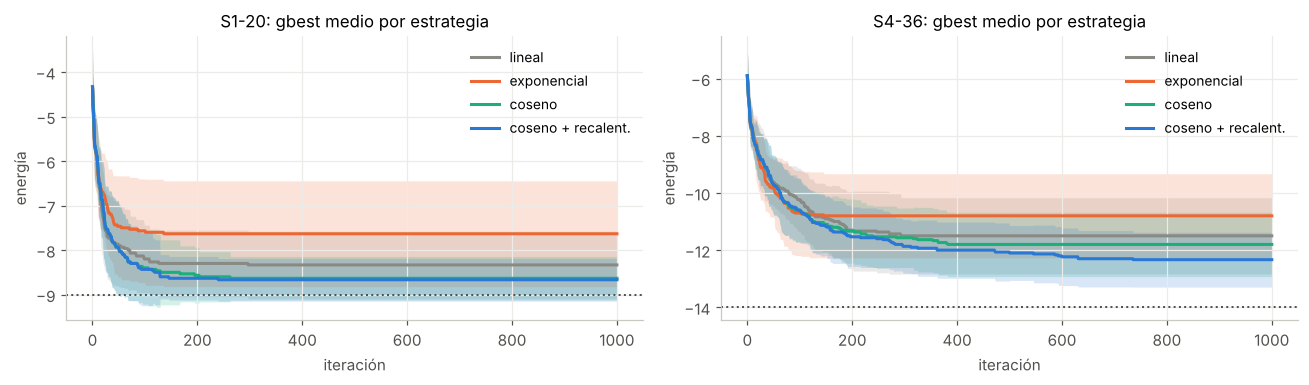
\includegraphics[width=\textwidth]{figuras/hp_comparacion_estrategias.png}
\caption{Convergencia media del \textit{gbest} con cada estrategia de coeficientes (30 ejecuciones). La banda es $\pm$ una desviación estándar.}
\label{fig:estrategias}
\end{figure}

La estrategia elegida tuvo la mejor media, la menor desviación estándar y el mayor número de éxitos en las dos cadenas. La diferencia contra la curva lineal y contra la exponencial es significativa en ambas ($p < 0.05$). Contra la curva coseno sin recalentamiento la diferencia es significativa en S4-36 ($p = 0.035$) pero no en S1-20 ($p = 0.398$). En S1-20 las dos versiones coseno tienen casi los mismos resultados (19 y 20 éxitos), porque la cadena es tan corta que el enjambre casi nunca se estanca lejos del óptimo y el recalentamiento tiene poco que hacer.

La curva exponencial fue la peor en las dos cadenas, con la media más alta y la mayor desviación estándar. En la Figura~\ref{fig:estrategias} se ve que su curva se aplana antes que las demás: en S4-36 casi no mejora después de la iteración 200. Al reducir $w$ y $c_1$ muy pronto, el enjambre se concentra en la primera región aceptable y ya no sale de ella. La curva lineal queda en medio, y el orden de las cuatro estrategias (exponencial, lineal, coseno, coseno con recalentamiento) coincide con el orden en que mantienen la exploración durante más tiempo.
